% *********************************************************************
% © 2021-2022 Jeremy Sylvestre
%
% Permission is granted to copy, distribute and/or modify this document
% under the terms of the GNU Free Documentation License, Version 1.3 or
% any later version published by the Free Software Foundation; with no
% Invariant Sections, no Front-Cover Texts, and no Back-Cover Texts. A
% copy of the license is included in the appendix entitled “GNU Free
% Documentation License” that appears in the output document of this
% PreTeXt source code. All trademarks™ are the registered® marks of
% their respective owners.
%
% *********************************************************************

\newcommand*{\xmin}{-5}
\newcommand*{\xmax}{25}
\newcommand*{\ymin}{-5}
\newcommand*{\ymax}{55}

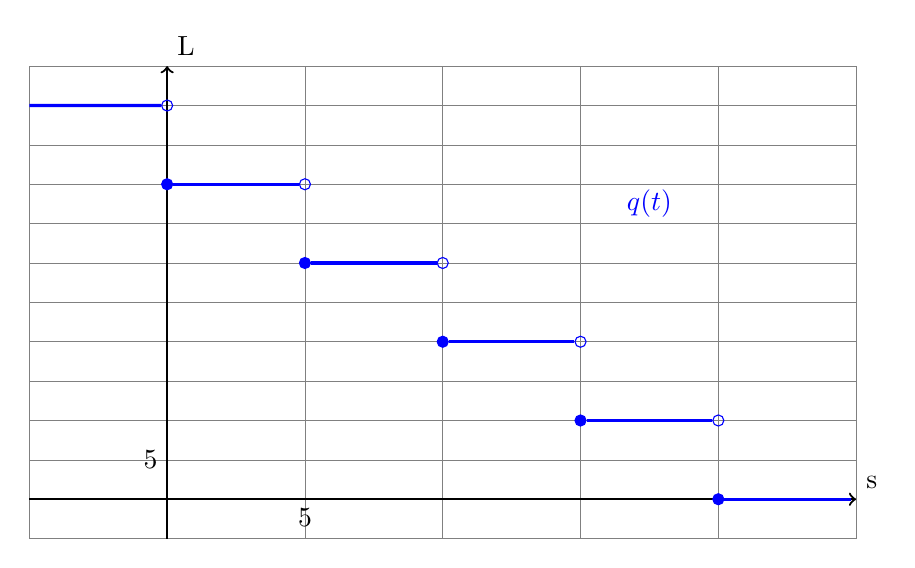
\begin{tikzpicture}
[
	closedpt/.style={circle,draw,fill,inner sep=0pt,minimum size=4pt},
	openpt/.style={circle,draw,inner sep=0pt,minimum size=4pt},
	xscale=0.35,
	yscale=0.1
]

	% grid
	\foreach \x in {\xmin,0,5,...,\xmax} {
		\draw[very thin,gray] (\x,\ymin) -- (\x,\ymax);
	}
	\foreach \y in {\ymin,0,5,...,\ymax} {
		\draw[very thin,gray] (\xmin,\y) -- (\xmax,\y);
	}

	% label grid
	\foreach \x in {5} {
		\node[below] at (\x,0) {$\x$};
	}
	\foreach \y in {5} {
		\node[left] at (0,\y) {$\y$};
	}

	% axes
	\draw[->,thick] (\xmin,0) -- (\xmax,0) node[above right] {s};
	\draw[->,thick] (0,\ymin) -- (0,\ymax) node[above right] {L};

	\node[openpt, blue] at (0,50) (end) {};
	\draw[blue, very thick] (-5,50) -- (end);

	\node[closedpt, blue] at (0,40) (start) {};
	\node[openpt, blue] at (5,40) (end) {};
	\draw[blue, very thick] (start) -- (end);

	\node[closedpt, blue] at (5,30) (start) {};
	\node[openpt, blue] at (10,30) (end) {};
	\draw[blue, very thick] (start) -- (end);

	\node[closedpt, blue] at (10,20) (start) {};
	\node[openpt, blue] at (15,20) (end) {};
	\draw[blue, very thick] (start) -- (end);

	\node[closedpt, blue] at (15,10) (start) {};
	\node[openpt, blue] at (20,10) (end) {};
	\draw[blue, very thick] (start) -- (end);

	\node[closedpt, blue] at (20,0) (start) {};
	\draw[blue, very thick] (start) -- (24.8,0);

	\node[blue, very thick] at (17.5,37.5) {$q(t)$};

\end{tikzpicture}
